%%%%%%%%%%%%%%%%%%%%%%%%%%%%%%%%%%%%%%%%%%%%%%%%%%%%%%%%%%%%%%%%%%%%%%%%%%%%%%%%%%%%%%
% Modelo de relatório de Disciplina de MLP a partir da
% classe latex iiufrgs disponivel em http://github.com/schnorr/iiufrgs
%%%%%%%%%%%%%%%%%%%%%%%%%%%%%%%%%%%%%%%%%%%%%%%%%%%%%%%%%%%%%%%%%%%%%%%%%%%%%%%%%%%%%%

%%%%%%%%%%%%%%%%%%%%%%%%%%%%%%%%%%%%%%%%%%%%%%%%%%%%%%%%%%%%%%%%%%%%%%%%%%%%%%%%%%%%%%
% Definição do tipo / classe de documento e estilo usado
%%%%%%%%%%%%%%%%%%%%%%%%%%%%%%%%%%%%%%%%%%%%%%%%%%%%%%%%%%%%%%%%%%%%%%%%%%%%%%%%%%%%%%
%
\documentclass[rel_mlp]{iiufrgs}

%%%%%%%%%%%%%%%%%%%%%%%%%%%%%%%%%%%%%%%%%%%%%%%%%%%%%%%%%%%%%%%%%%%%%%%%%%%%%%%%%%%%%%
% Importação de pacotes
%%%%%%%%%%%%%%%%%%%%%%%%%%%%%%%%%%%%%%%%%%%%%%%%%%%%%%%%%%%%%%%%%%%%%%%%%%%%%%%%%%%%%%
% (a A seguir podem ser importados os pacotes necessários para o documento, de acordo
% com a necessidade)
%
\usepackage[brazilian]{babel}	    % para texto escrito em pt-br
\usepackage[utf8]{inputenc}         % pacote para acentuação
\usepackage{graphicx}         	    % pacote para importar figuras
\usepackage[T1]{fontenc}            % pacote para conj. de caracteres correto
\usepackage{times}                  % pacote para usar fonte Adobe Times
\usepackage{enumerate}              % para lista de itens com letras
\usepackage{breakcites}
\usepackage{titlesec}
\usepackage{enumitem}
\usepackage{titletoc}
\usepackage{listings}			    % para listagens de código-fonte
\usepackage{mathptmx}               % p/ usar fonte Adobe Times nas formulas matematicas
\usepackage{url}                    % para formatar URLs
%\usepackage{color}				    % para imagens e outras coisas coloridas
%\usepackage{fixltx2e}              % para subscript
%\usepackage{amsmath}               % para \epsilon e matemática
%\usepackage{amsfonts}
%\usepackage{setspace}			    % para mudar espaçamento dos parágrafos
%\usepackage[table,xcdraw]{xcolor}  % para tabelas coloridas
%\usepackage{longtable}             % para tabelas compridas (mais de uma página)
%\usepackage{float}
%\usepackage{booktabs}
%\usepackage{tabularx}
%\usepackage[breaklinks]{hyperref}

\usepackage[alf,abnt-emphasize=bf]{abntex2cite}	% pacote para usar citações abnt
\usepackage[linesnumbered,ruled]{algorithm2e}
\usepackage{amsmath}



%%%%%%%%%%%%%%%%%%%%%%%%%%%%%%%%%%%%%%%%%%%%%%%%%%%%%%%%%%%%%%%%%%%%%%%%%%%%%%%%%%%%%%
% Macros, ajustes e definições
%%%%%%%%%%%%%%%%%%%%%%%%%%%%%%%%%%%%%%%%%%%%%%%%%%%%%%%%%%%%%%%%%%%%%%%%%%%%%%%%%%%%%%
%

% define estilo de parágrafo para citação longa direta:
\newenvironment{citacao}{
    %\singlespacing
    %\footnotesize
    \small
    \begin{list}{}{
        \setlength{\leftmargin}{4.0cm}
        \setstretch{1}
        \setlength{\topsep}{1.2cm}
        \setlength{\listparindent}{\parindent}
    }
    \item[]}{\end{list}
}

% adiciona a fonte em figuras e tabelas
\newcommand{\fonte}[1]{\\Fonte: {#1}}

% Ative o seguinte caso alguma nota de rodapé fique muito longa e quebre entre múltiplas
% páginas
%\interfootnotelinepenalty=10000

%%%%%%%%%%%%%%%%%%%%%%%%%%%%%%%%%%%%%%%%%%%%%%%%%%%%%%%%%%%%%%%%%%%%%%%%%%%%%%%%%%%%%%
% Informações gerais
%%%%%%%%%%%%%%%%%%%%%%%%%%%%%%%%%%%%%%%%%%%%%%%%%%%%%%%%%%%%%%%%%%%%%%%%%%%%%%%%%%%%%%

% título
\title{Modelos de Linguagens de Programação - SchnorR Doidão: Galáxias em R}

% autor
\author{Martinez}{José Pedro}
\author{Assis}{Lucas}
\author{Oberderfer}{Réges}


% Professor orientador da disciplina
\advisor[Prof.~Dr.]{Mello Schnorr}{Lucas}

% Nome do(s) curso(s):
\course{Curso de Graduação em Ciência da Computa{\c{c}}{\~a}o}

% local da realização do trabalho
\location{Porto Alegre}{RS}

% data da entrega do trabalho (mês e ano)
\date{12}{2017}


% Palavras chave
\keyword{Palavra-chave1}
\keyword{Palavra-chave2}
\keyword{Palavra-chave3}


%%%%%%%%%%%%%%%%%%%%%%%%%%%%%%%%%%%%%%%%%%%%%%%%%%%%%%%%%%%%%%%%%%%%%%%%%%%%%%%%%%%%%%
% Início do documento e elementos pré-textuais
%%%%%%%%%%%%%%%%%%%%%%%%%%%%%%%%%%%%%%%%%%%%%%%%%%%%%%%%%%%%%%%%%%%%%%%%%%%%%%%%%%%%%%

% Declara início do documento
\begin{document}

% inclui folha de rosto
\maketitle

\selectlanguage{brazilian}

% Sumario
\tableofcontents



%%%%%%%%%%%%%%%%%%%%%%%%%%%%%%%%%%%%%%%%%%%%%%%%%%%%%%%%%%%%%%%%%%%%%%%%%%%%%%%%%%%%%
% Aqui comeca o texto propriamente dito
%%%%%%%%%%%%%%%%%%%%%%%%%%%%%%%%%%%%%%%%%%%%%%%%%%%%%%%%%%%%%%%%%%%%%%%%%%%%%%%%%%%%%

%espaçamento entre parágrafos
%\setlength{\parskip}{6 pt}

\selectlanguage{brazilian}



%%%%%%%%%%%%%%%%%%%%%%%%%%%%%%%%%%%%%%%%%%%%%%%%%%%%%%%%%%%%%%%%%%%%%%%%%%%%%%%%%%%%%
% Introdução
%
\chapter{Introdução}

O presente trabalho consiste na implementação de um problema em dois paradigmas diferentes: funcional e orientado a objeto. A linguagem a ser utilizada deve ser a mesma para ambos os paradigmas.

O objetivo deste trabalho consiste em fornecer aos alunos a oportunidade de estudar uma linguagem de programação moderna com características híbridas (i.e., multiparadigma). O trabalho permitirá aos alunos demonstrarem que aprenderam os princípios de programação relacionados com os diferentes paradigmas estudados ao longo do semestre, demonstrando, ainda, a capacidade de analisar e avaliar linguagens de programação, seguindo os critérios abordados em aula.

As implementações, tanto funcional quanto orientada a objeto, e relatório estão disponíveis em \url{https://github.com/lbassis/galaxias}.
\section{Linguagem Escolhida: R}
	R é um projeto GNU \cite{GNU} voltado a programação estatística e gráfica. Faz parte dele uma linguagem multiparadigma (vetorial, orientada a objetos, imperativa, funcional, procedural e reflexiva) com tipagem dinâmica, fundamentada por S e inspirada por Scheme.

	A linguagem fornece uma grande variedade de ferramentas para estatística, como modelagem linear e não-linear, classificação, clustering, testes estatísticos. Um dos seus pontos fortes é a facilidade com que gráficos bem construídos e prontos para uso em publicações científicas podem ser gerados. Esses gráficos incluem formulas e símbolos matemáticos onde necessário.

	Resumindo, R é um conjunto integrado de métodos para manipulação de dados, cálculos e display gráfico que inclui \cite{linguagemR}:
\begin{itemize}
\item Uma série de operações sobre vetores, em particular matrizes;
\item Uma extensa coleção de ferramentas intermediárias para análise de dados;
\item Ferramentas de plot para análise de dados.
\item Uma linguagem de programação bem desenvolvida, simples e eficaz que inclui condicionais, loops, funções recursivas definidas pelo usuário e funções de entrada e saída.
\end{itemize}

\section{Problema escolhido: Galáxias}

	O problema consiste em implementar um simulador de partículas, considerando forças físicas de repulsão e atração. Serão utilizadas leis gravitacionais para simular órbitas de estrelas e planetas. Além disso, uma interface será criada para que seja possível acompanhar o movimento simulado.

    Para suportar a simulação de muitos corpos, será utilizado o algoritmo de Barnes-Hut \cite{Barnes}, que consiste em subdividir o espaço em quadrantes (no caso de um espaço bi-dimensional) recursivamente até atingir um dado limite de modo a simplificar o problema sem perdas consideráveis de precisão no modelo.

\subsection{Problema de N-corpos}

\begin{equation}
\label{theta}
\theta=\frac{d}{r}
\end{equation}

Uma determinada região do espaço contém N corpos, cada um com suas próprias propriedades como sua massa e com um campo de forças gravitacionais resultante agindo sobre si. A massa de cada corpo é uma característica física, e o campo resultante pode ser calculado a partir das posições dos corpos e de suas massas. Segundo a primeira lei de Newton, os corpos sofrem uma aceleração devido ao campo de forças gravitacionais resultante. Logo, a aceleração de um corpo e a sua posição dependem do campo de força resultante da interação entre todos os corpos.

Numa simulação desse problema, parte-se de um estado \textit{s} em que as posições e as velocidades dos corpos são conhecidas. A partir de \textit{s}, calculam-se as forças entre todos os corpos seguindo a equação \ref{forceEq}, onde $G$ é igual à constante gravitacional universal, $m_1$ é a massa do corpo 1, $m_2$ é a massa do corpo 2 e $r$ é a distância entre os dois corpos. Visto que é necessário calcular o campo de forças resultante para cada um dos corpos, $\frac{1}{2}N*(N-1)$ forças são calculadas. Logo, a complexidade de calcular todas as forças é $O(N^2)$.

\begin{equation}
\label{forceEq}
F=G\frac{m_1.m_2}{r^2}
\end{equation}

Uma vez que as forças foram calculadas, as acelerações das partículas são obtidas seguindo a equação \ref{accelerationEq}. Para o cálculo das novas posições e velocidades das partículas, assume-se um tempo $\Delta t$ entre cada etapa da simulação. Também se asssume que $\Delta t$ é suficientemente pequeno para que se possa fazer a aproximação que a aceleração é constante durante esse período de tempo. Utilizam-se, pois, as equações \ref{velocityEq} e \ref{positionEq} do Movimento Uniformemente Variado (MUV) para atualizar as posições e as velocidades das partículas.

\begin{equation}
\label{accelerationEq}
a=\frac{F}{m}
\end{equation}

\begin{equation}
\label{velocityEq}
v_{prox} = v_{atual} + a*\Delta t
\end{equation}

\begin{equation}
\label{positionEq}
s_{prox} = s_{atual} + v_{atual}*\Delta t + \frac{a}{2}*(\Delta t)^2
\end{equation}

\subsection{Algoritmo de Barnes-Hut}

O algoritmo de Barnes-Hut resolve o problema de N-corpos numa complexidade inferior àquela apresentada na seção anterior. Em vez de calcular todas as forças, uma aproximação baseada em árvores que divide o espaço em quadrantes é utilizada. Esse algoritmo tem complexidade igual a $O(N\,log(N))$

O algoritmo de Barnes-Hut reduz o número de forças calculadas agrupando partículas. A aproximação utilizada é que um grupo de partículas distantes pode ser reduzido a uma única partícula de centro igual ao centro de massa do grupo. Dessa forma, só é necessário calcular as forças uma a uma para partículas muito próximas, enquanto que as distantes têm seu cálculo simplificado. A simplificação só é válida quando a distância da partícula ao grupo é grande em relação ao tamanho do quadrante do grupo. Para determinar se a razão entre o tamanho $d$ do quadrante do grupo e a distância $r$ é suficiente, utiliza-se o critério da equação \eqref{theta}. O algoritmo de Barnes-Hut aplica $\theta=1$ subdividindo recursivamente o espaço em quadrantes até que apenas uma partícula por quadrante exista, como visto na Figura \ref{fig:barneshut.eps}.



\begin{figure}[htb]
    \centering
    \caption{Visualização do algoritmo de Barnes-Hut}
    \fbox{
        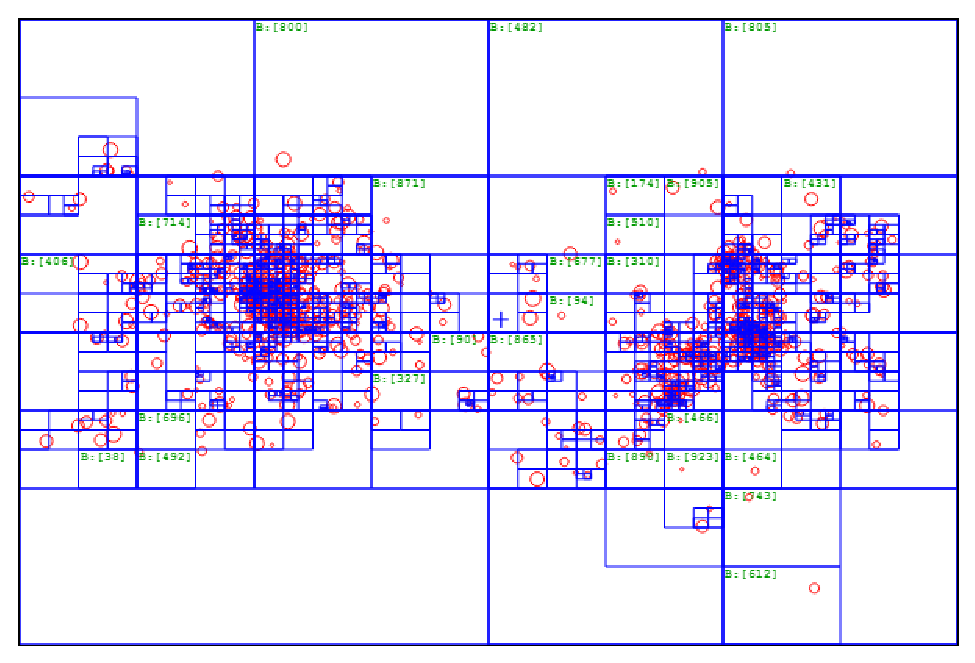
\includegraphics[width=20cm,height=10cm,keepaspectratio]{images/barneshut.eps}
    }
    \fonte{\cite{barnesHutImg}}
    \label{fig:barneshut.eps}
\end{figure}


\chapter{Implementação}

\section{Implementação Física}

O algoritmo recebe como entrada uma lista de partículas com suas posições e suas velocidades. Começa-se subdivindindo o espaço recursivamente em quadrantes até que haja no máximo uma partícula por quadrante. Ao mesmo tempo que os quadrantes são divididos, popula-se uma $QuadTree$ hierarquicamente de modo que cada nodo folha seja uma partícula do espaço, como pode ser visto na Figura \ref{fig:quadtree.eps}. Em um segundo momento, os centros de massa para cada quadrante são calculados. Após isso, calculam-se as forças resultantes para todas as partículas, reduzindo o número de forças calculadas quando um quadrante passa na regra da equação \eqref{theta}. Finalmente, as posições e velocidades das partículas são atualizadas considerando um passo de atualização que corresponde ao tempo percorrido entre uma etapa da simulação e a seguinte. A implementação em pseudocódigo pode ser vista no algoritmo \ref{barnesHutAlgorithm}.


\begin{figure}[htb]
    \centering
    \caption{Distribuição das partículas em seus quadrantes e $QuadTree$ correspondente.}
    \fbox{
        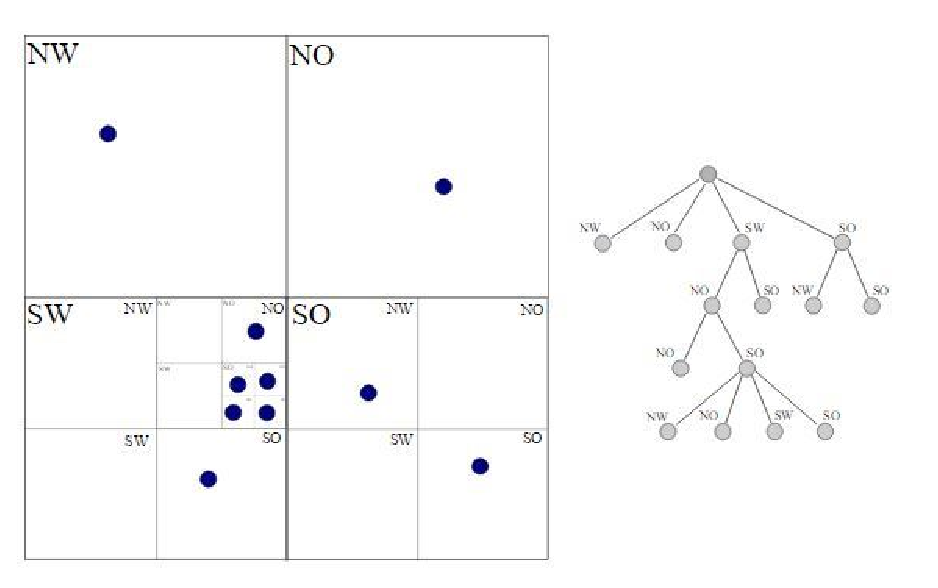
\includegraphics[width=20cm,height=10cm,,keepaspectratio]{images/quadtree.eps}
    }
    \label{fig:quadtree.eps}
    \fonte{\cite{galaxySimulator}}
\end{figure}


\begin{algorithm}
	\label{barnesHutAlgorithm}
    \SetKwInOut{Input}{Input}
    \SetKwInOut{Output}{Output}

    \underline{function barnesHut} $(particles, positions, velocities, masses)$\;
    \Input{Uma lista de partículas, suas posições, velocidades e massas}
    \Output{As posições e velocidades das partículas atualizadas}
    $quadTree = createQuadTree(particles, positions, velocities, masses)$\;
    $quadTree = computeMassDistribution(quadTree)$\;
    $quadTree = computeResultantForces(quadTree)$\;
    $newVelocities = updateVelocities(quadTree)$\;
    $newPositions = updatePositions(quadTree)$\;
    return $[newVelocities, newPositions]$\;
    \caption{Algoritmo de Barnes-Hut para simulação de N-corpos}
\end{algorithm}

\section{Implementação no Paradigma Funcional}

\subsection{Visualização Gráfica}

	A visualização gráfica foi implementada utilizando o pacote \textit{plotrix} e a biblioteca \textit{ImageMagick}. Em cada iteração do algoritmo, isto é, em cada conjunto de posições calculado, gera-se um gráfico com círculos representando as partículas em um espaço bidimensional, conforme é mostrado na figura \ref{fig:particulas.eps}.
    Em uma abordagem inicial, a ideia foi utilizar diversos gráficos carregados em sequência no ambiente \textit{Rstudio}, com um pequeno intervalo de espera entre cada geração. No entanto, a performance não foi satisfatória; apesar de, inicialmente e com um número pequeno de partículas, a animação ficasse fluída, com o passar do tempo o tempo entre as gerações é cada vez maior, tornando o algoritmo muito lento em pouco tempo.

    A partir daí, a ideia escolhida foi a de selecionar inicialmente um número de iterações; depois disso, são geradas todas as imagens necessárias para representar esse número e, por fim, as imagens são transformadas em um arquivo \textit{.gif}. Dessa maneira, o algoritmo perde a capacidade de ser demonstrado em tempo real, já que a duração da simulação é definida antes da execução da mesma. No entanto, dessa maneira foi possível obter uma animação adequada ao esperado e, portanto, essa foi a solução escolhida.

    A geração das imagens implementa um laço utilizando recursão. Enquanto um número de iterações (passado por parâmetro para a função) não for nulo, a recursão é chamada, reduzindo em uma unidade o número de iterações.
    Dentro do laço, uma partícula é desenhada utilizando a função \textit{draw{\_}circle}, implementadas conforme mostrado no algoritmo \ref{draw_particle}. Depois disso, uma função \textit{lapply} mapeia esse algoritmo para que ele seja aplicado a todas as partículas de uma lista, desenhando todos os elementos.
    Ao final da execução do laço, uma funçao da biblioteca \textit{ImageMagick} transforma as imagens geradas em um arquivo \textit{.gif} animado.

\begin{figure}[htb]
    \centering
    \caption{Visualização das partículas em um grafo}
    \fbox{
        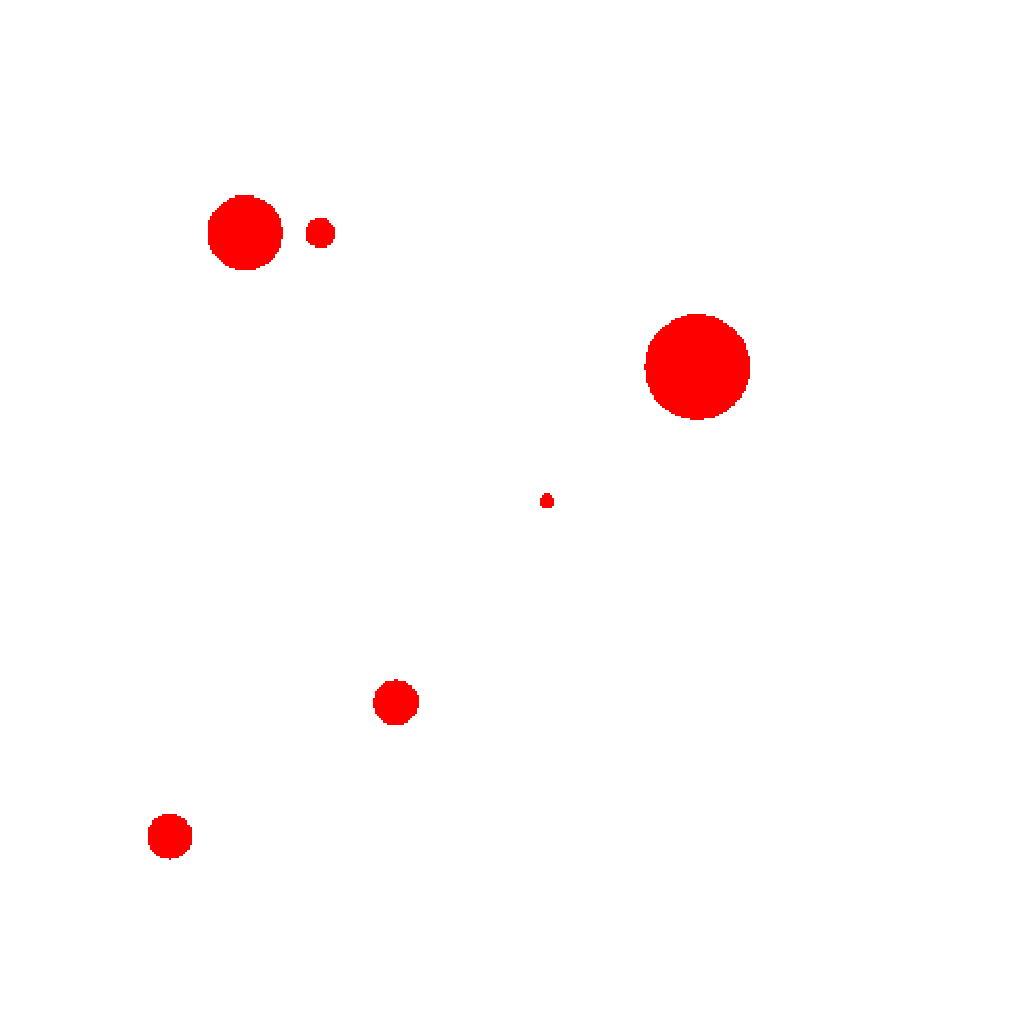
\includegraphics[width=20cm,height=10cm,,keepaspectratio]{images/particulas.eps}
    }
    \label{fig:particulas.eps}
\end{figure}


\begin{algorithm}
	\label{draw_particle}
    \SetKwInOut{Input}{Input}
    \underline{function draw{\_}particle} $(particle)$\;
    \Input{Uma partícula encapsulada em uma estrutura de nodo}
  	$	draw{\_}circle(qnode{\_}x(node), qnode{\_}y(node), qnode{\_}mass (node), col="red", nv=1000, border = NA,lty=1,lwd=1) $\;
    \caption{Algoritmo que desenha uma partícula}
\end{algorithm}

\section{Aspectos funcionais}

	Segue abaixo a descrição e demonstração de algumas técnicas tipicamente funcionais utilizadas na elaboração deste trabalho.

    \subsection{Elementos imutáveis}

    A utilização de elementos imutáveis é recorrente na solução desenvolvida. Como exemplo, pode-se citar a função de atualização da posição de uma partícula. A cada iteração do laço, uma nova partícula é criada (e, consequentemente, uma nova lista de partículas) para que esta ocupe a nova posição calculada com a velocidade também atualizada. A função que cria a nova partícula é mostrada no algoritmo \ref{particle_setPositionAndVelocity}.

    \begin{algorithm}
	\label{particle_setPositionAndVelocity}
    \SetKwInOut{Input}{Input}
    \SetKwInOut{Output}{Output}
    \underline{particle{\_}setPositionAndVelocity} $(particle, point, velocity)$\;
    \Input{Uma partícula e dois novos pontos representando sua nova posição e nova velocidade}
    \Output{Uma nova partícula criada com os parâmetros atualizados}
  		$particle{\_}setPositionAndVelocity <- function (particle, point, velocity) $\;
    	$new{\_}particle(point, qnode{\_}mass(particle), velocity, $\;
        $new{\_}point(qnode{\_}fx(particle), qnode{\_}fy(particle)), qnode{\_}size(particle)) $\;
\caption{Algoritmo de atualização de posição}
\end{algorithm}

    \subsection{Funções não nomeadas}

    Funções não nomeadas são utilizadas frequentemente para que elas possam ser passadas como se fossem um elemento de primeira ordem da implementação. Neste trabalho, por exemplo, foram utilizadas para definir a função da velocidade em função do tempo e da distância, demonstrada no algoritmo \ref{updateVelocityAndPosition} que é aplicada posteriormente nas componentes horizontal e vertical da velocidade de uma partícula.

    \begin{algorithm}
	\label{updateVelocityAndPosition}
    \SetKwInOut{Input}{Input}
    \SetKwInOut{Output}{Output}
    \underline{updateVelocityAndPosition} $(node, deltaT)$\;
    \Input{Uma partícula encapsulada em um nodo e um intervalo de tempo a ser considerado}
    \Output{Uma nova partícula criada com os parâmetros atualizados}
  		$calcVelocityComponent <- function (v, a, t) (v + a*t)$\;
    	$newVx <- calcVelocityComponent(vx, ax, deltaT)$\;
    	$newVy <- calcVelocityComponent(vy, ay, deltaT)$\;

\caption{Trecho do algoritmo do cálculo da nova posição}
\end{algorithm}

	\subsection{Currying}

    O \textit{Currying} é uma técnica que transforma uma função de duas entradas em uma função com uma entrada que retorna outra função de uma entrada. Nesse trabalho, essa implementação foi utilizada para acessar as colunas dos \textit{data.frames} criados - os \textit{qnodes}. O algoritmo \ref{qnode_data} mostra a implementação da função "original".
    \begin{algorithm}
	\label{qnode_data}
    \SetKwInOut{Input}{Input}
    \SetKwInOut{Output}{Output}
    \underline{qnode{\_}data} $(data, node)$\;
    \Input{A descrição de uma coluna do dataframe e uma partícula encapsulada em um nodo}
    \Output{O valor associado à coluna selecionada no nodo fornecido}
	$if(is.data.frame(node)) $\;
    $node[data][[1]] $\;
  	$else if(!qnode{\_}empty(node)) $\;
    $node[[1]][data][[1]] $\;
  	$else 0 $\;
	\caption{Algoritmo seletor de colunas do dataframe node}
	\end{algorithm}

    A partir daí, torna-se fácil construir as funções específicas de cada seletor, que utilizam como argumento apenas o \textit{qnode} a ser acessado. Utilizando a função \textit{Curry} do pacote \textit{functional}, temos a seguinte implementação para obter o parâmetro \textit{point{\_}x}, por exemplo.

    \begin{algorithm}
	\label{qnode_x}
    \SetKwInOut{Input}{Input}
    \SetKwInOut{Output}{Output}
    \underline{qnode{\_}x} $(node)$\;
    \Input{Uma partícula encapsulada em um nodo}
    \Output{O valor da coluna x no nodo fornecido}
	$Curry(qnode{\_}data, data="point{\_}x") $\;
	\caption{Algoritmo seletor da coluna x do dataframe node}
	\end{algorithm}

	\subsection{Funções de ordem superior próprias}

    Funções de ordem superior aceitam que outras funções sejam passadas como parâmetro. Como exemplo, temos a implementação da funçao
        \textit{best{\_}point}, conforme visto na função \ref{best_point}. Para determinar os limites do gráfico e o centro geométrico da simulação,
         são computados o ponto mais à esquerda/mais acima e a maior distãncia em uma das dimensões até outro ponto pertencente à simulação. Tendo a função de alta ordem \textit{best{\_}point} e usando as funções primitivas min e max, é possível atualizar os limites \textit{top{\_}left} e \textit{bottom{\_}right} (este usado para atualizar a maior distância entre os pontos) recursivamente.

    \begin{algorithm}
    \label{best_point}
    \SetKwInOut{Input}{Input}
    \SetKwInOut{Output}{Output}
    \underline{best{\_}point} $(p, q, fun)$\;
    \Input{Um ponto, um quadrante e uma função para determinar o ponto mais apropriado}
    \Output{O ponto mais extremo do quadrante}
    $ new_point(fun(q["x"][[1]], p["x"][[1]]), fun(q["y"][[1]], p["y"][[1]])); $\;
    \caption{Algoritmo que encontra os extremos dos quadrantes}
    \end{algorithm}

    \subsection{Funções de ordem superior prontas}

    Um dos exemplos a ser citado de funções de ordem superior já implementadas pela linguagem é a função \textit{lapply}. Ela funciona como um funtor, mapeando uma função que recebe um elemento e generaliza-na para que ela receba uma lista desses elementos, aplicando a função inicial a todos eles. No algoritmo \ref{draw_particle}, por exemplo, desenha-se uma partícula. A partir dele, pode-se construir o algoritmo \ref{draw_particles}, generalizando sua implementação para trabalhar com uma lista de partículas em vez de um único elemento.

    \begin{algorithm}
	\label{draw_particles}
    \SetKwInOut{Input}{Input}
    \underline{draw{\_}particles} $(particles)$\;
    \Input{Uma lista de partículas encapsulada em nodos}
	$invisible(lapply(particles, draw{\_}particle)) $\;
	\caption{Algoritmo que desenha todas as partículas do instante atual}
	\end{algorithm}

	\subsection{Funções como elemento de primeira ordem}

    Em linguagens funcionais, é possível que funções sejam passadas como parâmetros de outras funções, funcionando como elementos de primeira ordem. Essa técnica foi utilizada no \textit{loop} que desenha as partículas para indicar qual a função que atualizaria suas posições, conforme mostrado no algoritmo \ref{drawing_loop}.

    \begin{algorithm}
	  \label{drawing_loop}
    \SetKwInOut{Input}{Input}
    \underline{drawing{\_}
loop} $(particles, iteractions, name, updatePosAndVel)$\;
    \Input{Uma lista de partículas encapsulada em nodos, o número de iterações do laço, o nome dos arquivos temporários e uma função que devolve uma lista de nodes}

  $if (iteractions == 0) $\;
  $  system("convert -delay 10 *.jpg result.gif") $\;
  $  file.remove(list.files(pattern=".jpg")) $\;
  $else $\;
  $  name <- paste(name, "a") $\;
  $  filename <- paste(name, ".jpg") $\;
  $  png(filename = filename) $\;
  $  plot.new() $\;
  $  frame() $\;
  $  draw{\_}particles(normalize{\_}masses(particles)) $\;
  $  dev.off() $\;
  $  particles <- updatePosAndVel(qList{\_}toParticles(particles)) $\;
  $  drawing{\_}loop(particles, iteractions-1, name, updatePosAndVel) $\;
    \caption{Laço que desenha os quadros da animação}
    \end{algorithm}

    \subsection{Funções com pattern matching}

    \textit{Pattern matching} é uma técnica que procura padrões dentro de sequências de valores, muito utilizada, por exemplo, em processamento de linguagens. Como esse trabalho é uma implementação que simula fenômenos físicos, o grupo não encontrou uma aplicação interessante para esse tipo de algoritmo, portanto não há nenhum exemplo a ser mostrado.

    \subsection{Recursão}

      A recursão foi utilizada frequentemente como iterador para que todos os elementos de uma lista
      fossem devidamente processados. Um possível exemplo é o algoritmo~\ref{drawing_loop}
      mostrado na sessão anterior. Ao final de cada iteração, diminui-se em uma unidade o número de iterações
      restantes e a função \textit{drawing{\_}loop} é chamada novamente.

\subsection{Análise do algoritmo}

O grupo teve dificuldade em encontrar valores de variáveis adequados para realizar as simulações. Portanto,
não foi gerado nenhum caso de teste grande o suficiente para comprovar a eficiência do algoritmo em relação
à uma solução em força bruta. Por isso, foi elaborado o gráfico \ref{fig:grafico} a partir do caso de teste elaborado, comparando
a quantidade de comparações do algoritmo de força bruta com a solução implementada. O eixo X representa o número
de partículas, enquanto o eixo Y representa o número de comparações.

\begin{figure}[htb]
    \centering
    \caption{Comparação força bruta com Barnes-Hut}
    \fbox{
        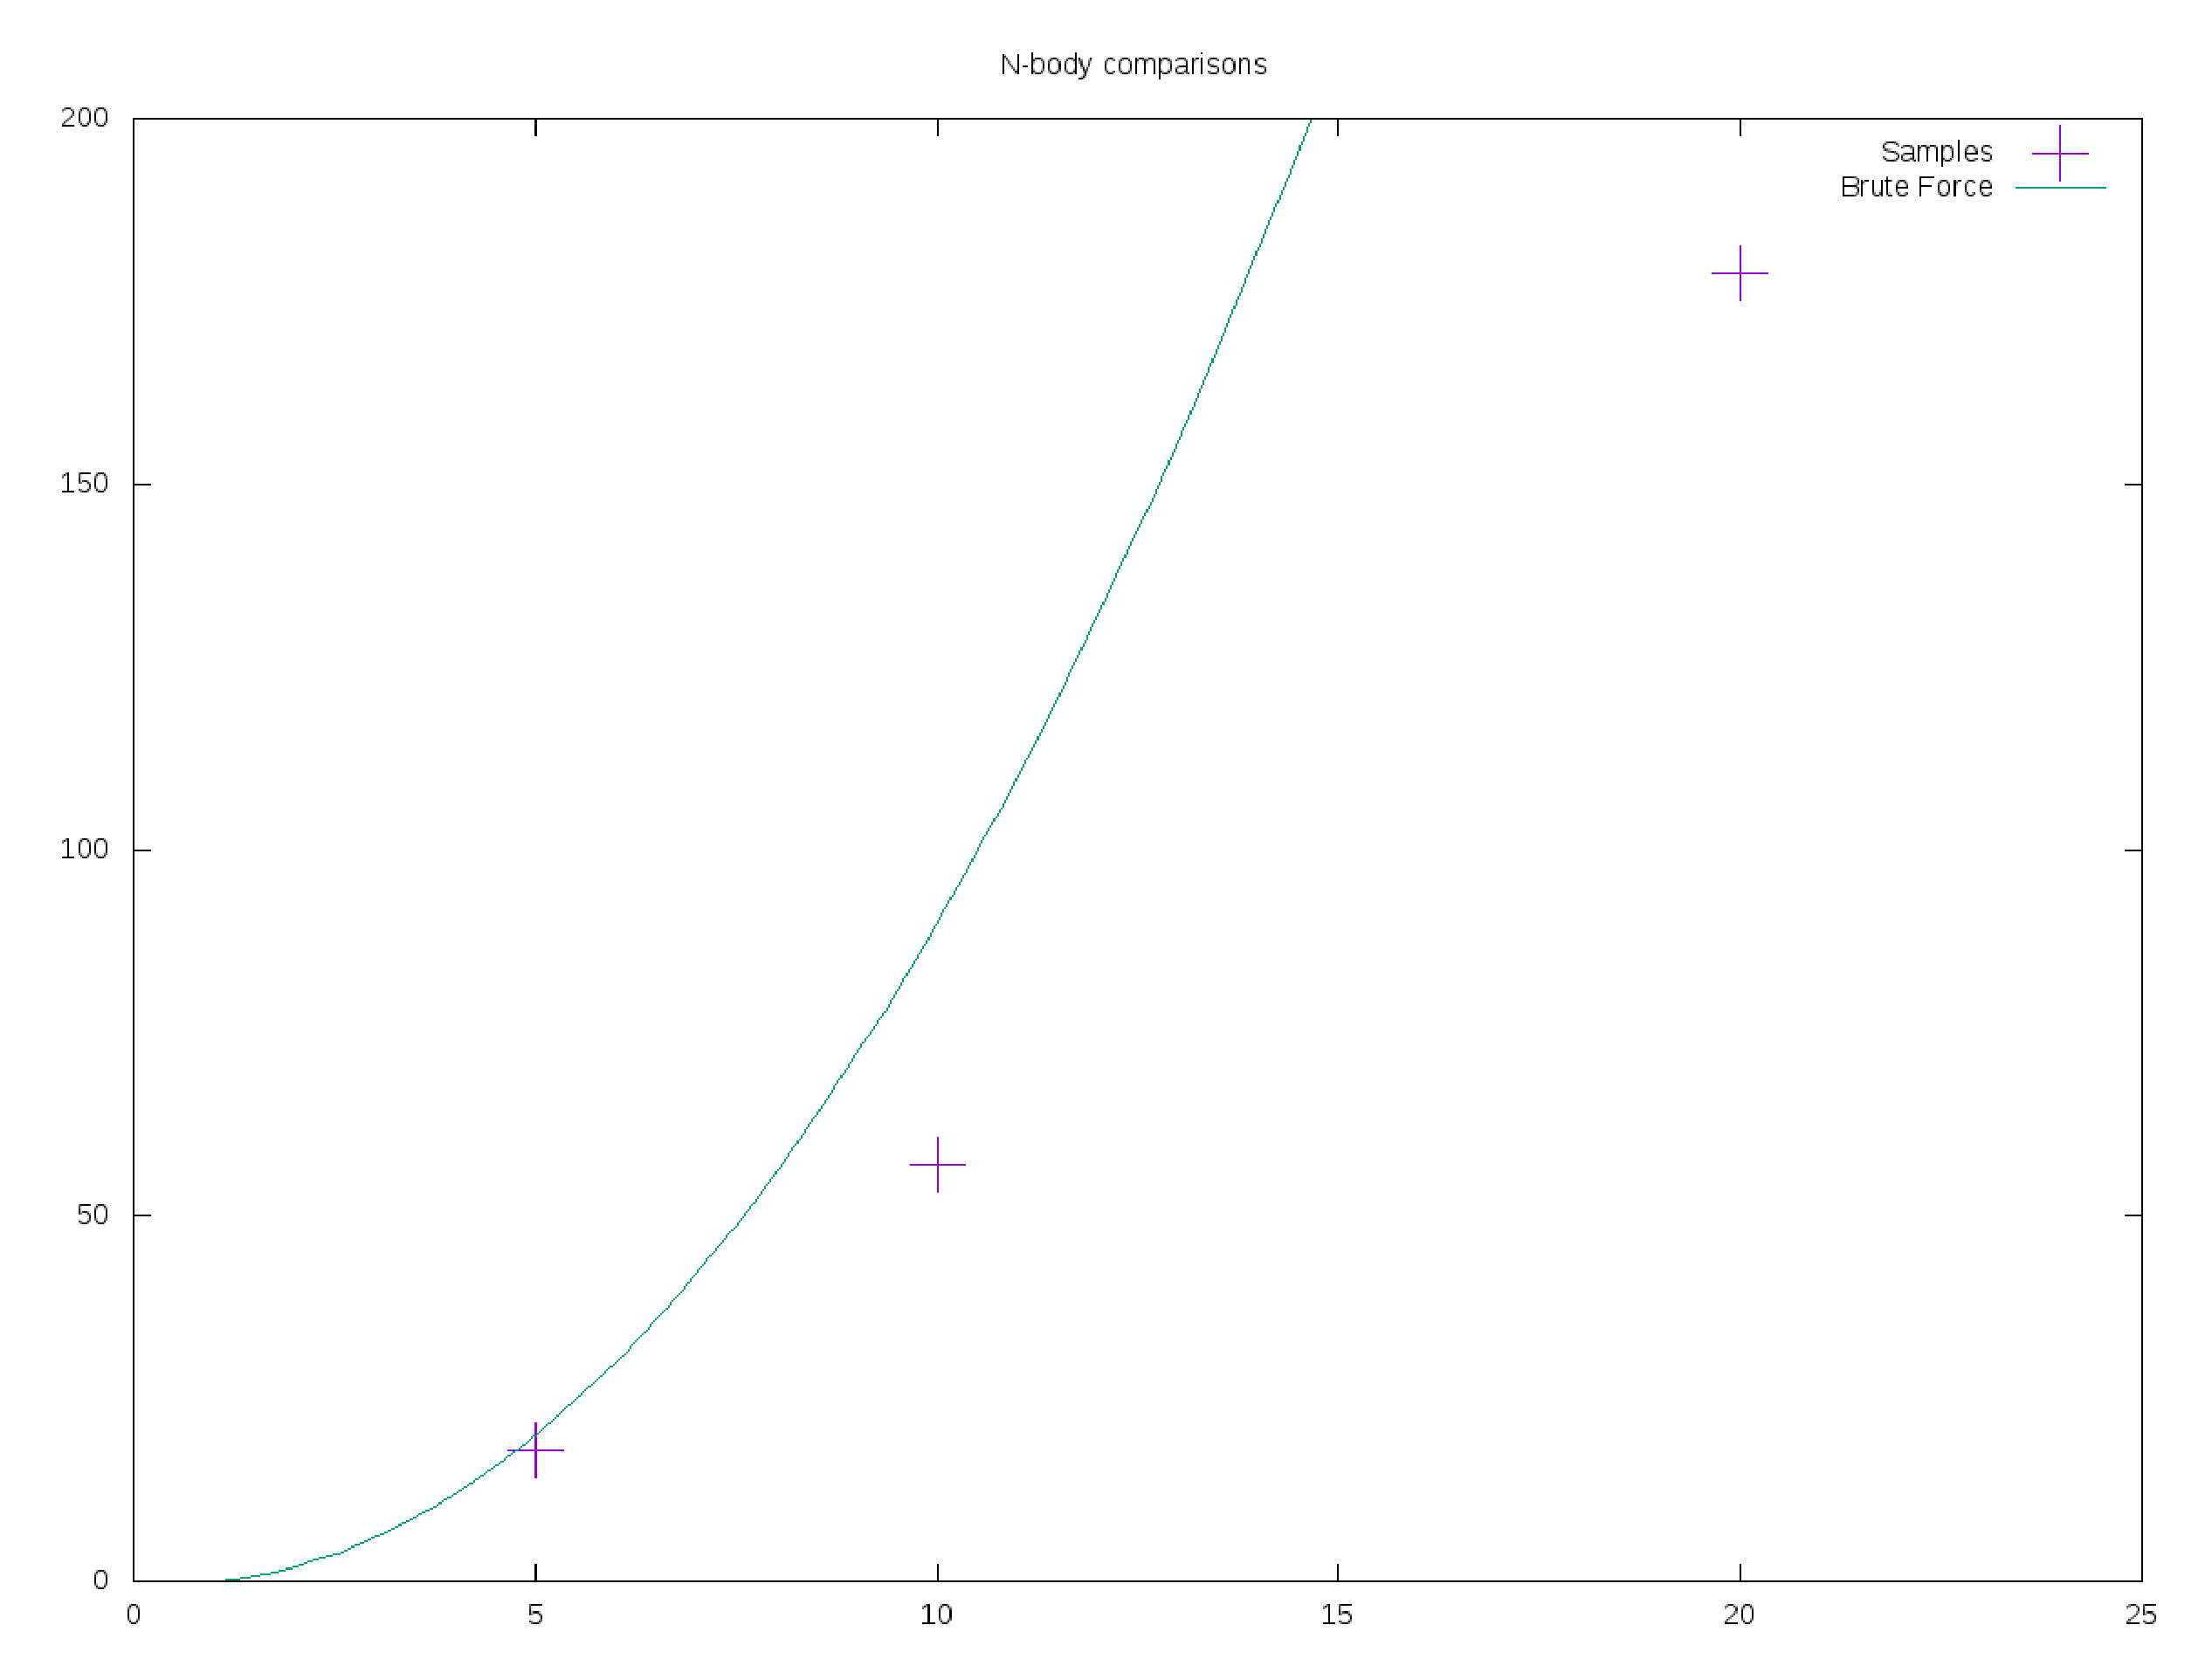
\includegraphics[width=20cm,height=10cm,keepaspectratio]{images/grafico.eps}
    }
    \label{fig:grafico}
\end{figure}



\subsection{Análise da linguagem}

A seguir são atribuídas notas às diferentes características da linguagem R quando considerando uma implementação usando o paradigma funcional. As notas foram dadas em um intervalo [0,5].


\begin{table}[ht]
  \caption{Características da linguagem R}
  \centering
    \begin{tabular}{ c | c }
        \hline
        \textit{Característica} &
        \textit{Nota [0, 5]} \\
        \hline
        Simplicidade & 3.5\\
        \hline
        Ortogonalidade & 4.5\\
        \hline
        Expressividade & 3.0\\
        \hline
        Adequabilidade e variedade de estruturas de controle & 4.0\\
        \hline
        Mecanismos de definição de tipos & 4.0\\
        \hline
        Suporte a abstração de dados & 3.0\\
        \hline
        Suporte a abstração de processos & 4.5\\
        \hline
        Modelo de tipos & 3.0\\
        \hline
        Portabilidade & 3.0\\
        \hline
        Reusabilidade & 4.5\\
        \hline
        Suporte e documentação & 3.0\\
        \hline
        Tamanho de código & 4.0\\
        \hline
        Generalidade & 3.0\\
        \hline
        Eficiência & 4.0\\
        \hline
        Custo & 2.5\\
      \hline
    \end{tabular}
     \fonte{Autor}
  \label{tab:caracteristicas}
\end{table}

A seguir, temos as análises que levaram a cada uma das notas mostradas na tabela.

\subsubsection{Simplicidade}
O operador <- vai contra a simplicidade da linguagem, já que ele implementa a atribuição, assim como o operador =.

\subsubsection{Ortogonalidade}
Diversas funções do programa alternam entre data.frames e listas, e a linguagem oferece suporte a isso naturalmente.

\subsubsection{Expressividade}
A expressividade é adequada no geral, porém no acesso à listas, a necessidade de usar dois colchetes para recuperar um elemento torna o código menos expressivo do que ele poderia ser. Como alternativa, temos as funções \textit{head} e \textit{tail}, porém as duas também contam com um fator incomum que é a necessidade de especificar quantos elementos serão recuperados da lista.

\subsubsection{Adequabilidade e variedade de estruturas de controle}
As estruturas de controle existem, mas a implementação funcional utiliza recursão em seu lugar. Apesar disso, alguns laços iterativos foram úteis para depuração do código.

\subsubsection{Mecanismos de definição de tipos}
O tipo data.frame, utilizado para representar tabelas, funciona como uma definição de estrutura e atendeu bem ao desejado no trabalho.

\subsubsection{Suporte a abstração de dados}
A linguagem fornece a estrutura data.frame, que equivale a uma tabela em que cada coluna pode ter um valor de diferentes tipos. No entanto, não é criada uma estrutura propriamente dita, com sua própria semântica.

\subsubsection{Suporte a abstração de processos}
Implementa funções recursivas e inclusive funções como elementos de primeira ordem, tornando o suporte a abstração de processos excelente.

\subsubsection{Modelo de tipos}
Sendo uma linguagem dinamicamente tipada, o modelo de tipos deixa a desejar. Em alguns casos, houveram problemas de difícil identificação que, com um sistema de tipos mais robusto, seriam facilmente detectáveis.

\subsubsection{Portabilidade}
A linguagem oferece diversos pacotes, mas todos os utilizados precisaram ser instalados posteriormente.

\subsubsection{Reusabilidade}
A utilização de funções como elementos de primeira ordem faz com que a linguagem possua uma ótima reusabilidade.

\subsubsection{Suporte e documentação}
Especialmente para este trabalho, que não utiliza a linguagem em um contexto em que ela se destaca, foi difícil encontrar referências para várias funcionalidades. No entanto, isso talvez esteja mais relacionado com a natureza da aplicação desenvolvida do que com a linguagem em si.

\subsubsection{Tamanho de código}
Nada especialmente diferente do comum. A linguagem não tem o código muito longo nem notoriamente curto.

\subsubsection{Generalidade}
Apesar de ter sido usada satisfatoriamente nesse trabalho, a linguagem fornece muito mais recursos para algoritmos estatísticos e similares do que qualquer outra implementação.

\subsubsection{Eficiência}
Para que essa característica seja analisada apropriadamente, seria necessário implementar o mesmo algoritmo em outro paradigma/linguagem, portanto fica difícil avaliar sem ao menos concluir a implementação orientada a objeto. No entanto, pode-se observar que a maior parte do tempo que o algoritmo leva é na criação dos arquivos de imagem, indicando que as funções próprias são eficientes.

\subsubsection{Custo}
A curva de aprendizado é relativamente íngreme; além disso, o Rstudio eventualmente apresenta problemas em sua instalação e na instalação de seus pacotes. Por fim, para uma simulação física como a aqui apresentada, as estruturas nativas da linguagem e do ambiente não facilitam, portanto conclui-se que nesse caso o custo é alto.



%%%%%%%%%%%%%%%%%%%%%%%%%%%%%%%%%%%%%%%%%%%%%%%%%%%%%%%%%%%%%%%%%%%%%%%%%%%%%%%%%%%%%
% Conclusões
%
\chapter{CONCLUSÃO}

Ao final deste trabalho, foi possível formar uma opinião sobre várias das construções da programação funcional que o grupo nunca havia implementado. No entanto, se tratando de uma simulação física, também foi confirmado que R não é a linguagem mais adequada para construir esse tipo de programa.
O algoritmo implementado demonstra uma possibilidade de simular diversas partículas com uma complexidade reduzida. Contudo, devido à dificuldade para gerar casos de teste, só foram criadas simulações com um número pequeno de partículas, não aproveitando o potencial total do algoritmo. Por esse motivo, o grupo optou por elaborar o gráfico que demonstra a eficiência do algoritmo em relação à uma implementação em força bruta.

Houve algumas dificuldades iniciais para definir as estruturas da implementação, já que foi necessário encapsular
as partículas juntamente com os subquadrantes.

Por fim, um problema que foi detectado no final da implementação foi que o grupo não implementou colisões.
Dessa maneira, assim que duas partículas ficam muito próximas uma da outra, as suas acelerações crescem até que elas sejam "arremessadas" com uma velocidade irreal. No entanto, até a conclusão da implementação
orientada a objeto, acredita-se que esse problema terá sido tratado.



%%%%%%%%%%%%%%%%%%%%%%%%%%%%%%%%%%%%%%%%%%%%%%%%%%%%%%%%%%%%%%%%%%%%%%%%%%%%%%%%%%%
% Referências
%%%%%%%%%%%%%%%%%%%%%%%%%%%%%%%%%%%%%%%%%%%%%%%%%%%%%%%%%%%%%%%%%%%%%%%%%%%%%%%%%%%
%
%\chapter{Referências}
\bibliographystyle{abntex2-alf}


\bibliography{biblio.bib} % arquivo que contém as referências (no formato bib). Colocar as suas lá (se tiver dúvida sobre como adicionar novas referências, usar o software JabRef ou Medley)

%\noindent SAMEER A. Barnes-Hut N-body Simulation in HTML/Javascript. Disponível em $<$https://github.com/Elucidation/Barnes-Hut-Tree-N-body-Implementation-in-HTML-Js$>$. Acesso em: nov. 2017.

%\noindent R: What is R? Disponível em $<$https://www.r-project.org/about.html$>$. Acesso em: nov. 2017.

%\noindent BERG I. The Barnes-Hut Galaxy Simulator. Disponível em $<$http://beltoforion.de/article.php?a=barnes-hut-galaxy-simulator$>$. Acesso em: nov. 2017.



\end{document}
